% Options for packages loaded elsewhere
\PassOptionsToPackage{unicode}{hyperref}
\PassOptionsToPackage{hyphens}{url}
%
\documentclass[
]{article}
\usepackage{amsmath,amssymb}
\usepackage{iftex}
\ifPDFTeX
  \usepackage[T1]{fontenc}
  \usepackage[utf8]{inputenc}
  \usepackage{textcomp} % provide euro and other symbols
\else % if luatex or xetex
  \usepackage{unicode-math} % this also loads fontspec
  \defaultfontfeatures{Scale=MatchLowercase}
  \defaultfontfeatures[\rmfamily]{Ligatures=TeX,Scale=1}
\fi
\usepackage{lmodern}
\ifPDFTeX\else
  % xetex/luatex font selection
\fi
% Use upquote if available, for straight quotes in verbatim environments
\IfFileExists{upquote.sty}{\usepackage{upquote}}{}
\IfFileExists{microtype.sty}{% use microtype if available
  \usepackage[]{microtype}
  \UseMicrotypeSet[protrusion]{basicmath} % disable protrusion for tt fonts
}{}
\makeatletter
\@ifundefined{KOMAClassName}{% if non-KOMA class
  \IfFileExists{parskip.sty}{%
    \usepackage{parskip}
  }{% else
    \setlength{\parindent}{0pt}
    \setlength{\parskip}{6pt plus 2pt minus 1pt}}
}{% if KOMA class
  \KOMAoptions{parskip=half}}
\makeatother
\usepackage{xcolor}
\usepackage[margin=1in]{geometry}
\usepackage{longtable,booktabs,array}
\usepackage{calc} % for calculating minipage widths
% Correct order of tables after \paragraph or \subparagraph
\usepackage{etoolbox}
\makeatletter
\patchcmd\longtable{\par}{\if@noskipsec\mbox{}\fi\par}{}{}
\makeatother
% Allow footnotes in longtable head/foot
\IfFileExists{footnotehyper.sty}{\usepackage{footnotehyper}}{\usepackage{footnote}}
\makesavenoteenv{longtable}
\usepackage{graphicx}
\makeatletter
\def\maxwidth{\ifdim\Gin@nat@width>\linewidth\linewidth\else\Gin@nat@width\fi}
\def\maxheight{\ifdim\Gin@nat@height>\textheight\textheight\else\Gin@nat@height\fi}
\makeatother
% Scale images if necessary, so that they will not overflow the page
% margins by default, and it is still possible to overwrite the defaults
% using explicit options in \includegraphics[width, height, ...]{}
\setkeys{Gin}{width=\maxwidth,height=\maxheight,keepaspectratio}
% Set default figure placement to htbp
\makeatletter
\def\fps@figure{htbp}
\makeatother
\setlength{\emergencystretch}{3em} % prevent overfull lines
\providecommand{\tightlist}{%
  \setlength{\itemsep}{0pt}\setlength{\parskip}{0pt}}
\setcounter{secnumdepth}{-\maxdimen} % remove section numbering
\usepackage{titling}
\pretitle{\begin{center}\Huge\bfseries}
\posttitle{\par\end{center}}
\predate{\begin{center}\large}
\postdate{\par\end{center}}
\preauthor{\begin{center}\large}
\postauthor{\par\end{center}}
\usepackage{amsmath}
\usepackage{amsthm}
\usepackage{rotating}
\ifLuaTeX
  \usepackage{selnolig}  % disable illegal ligatures
\fi
\usepackage{bookmark}
\IfFileExists{xurl.sty}{\usepackage{xurl}}{} % add URL line breaks if available
\urlstyle{same}
\hypersetup{
  pdftitle={Transit Usage in Seattle: A Spatial Investigation},
  pdfauthor={Peter Silverstein},
  hidelinks,
  pdfcreator={LaTeX via pandoc}}

\title{Transit Usage in Seattle: A Spatial Investigation}
\author{Peter Silverstein}
\date{2024-12-11}

\begin{document}
\maketitle

\begin{center}
    {\large Final Project}\\[0.5cm]
    {\large GIS and Spatial Analysis}\\[0.5cm]
    {\large QMSS5070}\\[0.5cm]
\end{center}

\newpage

\tableofcontents

\newpage

\section{Introduction}\label{introduction}

\subsection{Research Question:}\label{research-question}

\begin{enumerate}
\def\labelenumi{\arabic{enumi}.}
\tightlist
\item
  How does transit usage percentage (percent of trips using mass transit
  / total trips per census tract) vary spatially in and around Seattle
  and Tacoma, Washington?
\item
  How does this variation relate to population density, median income,
  and median age at the census tract level?
\end{enumerate}

\subsection{Purpose of Study:}\label{purpose-of-study}

There are essentially two purposes to this study. The first is to better
understand where there are concentrations of high and low transit usage
around the region. If there is clustering and we see hotspots and/or
coldspots, further policy-focused questions can be asked. For example:
given clustering, what characteristics of a census tract makes in more
or less likely to be in one of these hot or cold zones? How might we
allocate resources across hot zones, cold zones, and those in-between to
increase the adoption of transit by commuters? Is the dispersion of
transit availability closely related to the demand and does the
dispersion favor certain demographic groups over others?

The second research question is a very basic attempt at answering one of
these follow-up questions. By understanding how each of the three
independent variables (population density, median income, and median
age) are related to the outcome of interest (percentage of commuter
trips taken using public transit), we can begin to fill in the knowledge
gaps demonstrated by the questions above.

\subsection{Hypotheses}\label{hypotheses}

\begin{enumerate}
\def\labelenumi{\arabic{enumi}.}
\tightlist
\item
  I believe we will see transit hotspots close to urban centers (e.g.,
  Seattle and Tacoma, the two biggest cities in the region of interest).
  Further, I believe the opposite will be true for coldspots--they
  should exist further outside urban centers. These ideas are based on
  the fact that transit lines themselves tend to be clustered in
  high-density, urban areas, meaning opportunities for mass transit
  travel are more convenient and plentiful in more central urban areas.
\item
  I expect that transit use percentage is positively associated with
  population density and median income and negatively associated with
  age. I make this hypothesis about population density based on the
  reasoning above. I expect younger people to (a) be more likely to live
  in highly urban areas and (b) be less likely to own a personal vehicle
  (such as a car). Of the three variables, I am the least confident
  about median income, because I think the relationship could be pulled
  in both positive and negative directions. On one hand, urban areas
  tend to be more expensive and thus have a higher requirement for
  income to live there. On the other hand, lower income should be
  associated with lower rates of car ownership and thus lower income
  would be associated with higher transit ridership.
\end{enumerate}

\section{Data and Methodology:}\label{data-and-methodology}

\subsection{Data Sources:}\label{data-sources}

\begin{enumerate}
\def\labelenumi{\arabic{enumi}.}
\tightlist
\item
  The \textbf{Puget Sound Regional Association (PSRC) Household Travel
  Survey (HTS) 2017-23} is a biennial survey of commuters done in the
  King, Kitsap, Pierce, and Snohomish counties of Washington state (the
  counties surrounding Seattle and Tacoma). The present analysis uses
  the Trips dataset from the HTS. Each observation in the dataset
  represents a single trip taken by a respondent and includes a variety
  of variables. Most important for my analysis are origin/destination
  tract and mode of travel, although the dataset also includes date,
  time, distance, speed, etc.
\item
  All \textbf{census tract-level ACS 2022 5-year estimates for
  demographic data and the associated geometries} were accessed via the
  R \texttt{tidycensus} package, which leverages an API connection to
  the US Census Bureau to provide US Census data for a specified
  geographic area.
\item
  Finally, \textbf{Stanford's Cities and Towns of the United States,
  2014} dataset provided point data to allow me to add city labels to my
  maps for reference.
\end{enumerate}

\subsection{Data Preparation/Spatial Data
Management:}\label{data-preparationspatial-data-management}

\subsubsection{Data Cleaning}\label{data-cleaning}

The output from \texttt{tidycensus} is already quite clean, so the
majority of data cleaning steps were conducted on the PSRC HTS dataset.
After loading the dataset, I selected my columns of interest and
converted their types where appropriate and useful (e.g., string to
factor). The next step was to collapse the mode of travel column from
around 50 unique responses (an artifact of (a) a very detailed survey
and (b) some changes to response options over the years) to just 4
useful categories, outlined below:

\begin{enumerate}
\def\labelenumi{\arabic{enumi}.}
\tightlist
\item
  \emph{Mass Transit:} included in this category trips that used a metro
  bus, private bus or shuttle, urban rail/light rail, school bus, ferry,
  paratransit, and commuter rail. Essentially I included any
  multi-occupancy transit vehicle.
\item
  \emph{Personal Vehicle:} trips including all single-occupancy motor
  vehicles. This includes personal cars, ride-shares, taxis,
  motorcycles, and car-share services.
\item
  \emph{Active Transit:} included walking, running, biking, and
  skateboarding.
\item
  \emph{Other:} included helicopter/plane, ``other'' responses.
\end{enumerate}

I then implemented a number of filters to filter data that either didn't
seem realistic or were outside the scope of this question. This included
the following operations:

\begin{enumerate}
\def\labelenumi{\arabic{enumi}.}
\tightlist
\item
  Filtered non-complete survey responses
\item
  Filtered distance to the range of 0 to 150 miles
\item
  Filtered trip duration to only include those greater than 0 minutes
\item
  Filtered speed to exclude speeds greater than 150 mph
\item
  Filtered to remove observations with missing value for travel mode
\end{enumerate}

\subsubsection{Spatial Joins}\label{spatial-joins}

The next step was to count the number of trips and join these values to
the geometries/ACS data from tidyverse. I used the \texttt{summarize()}
function to count the number of total trips and number of trips per
category for each census tracts. I then joined these counts to my
geometry table via the \texttt{left\_join()} function and matched on
GEOID. Further, I removed any tracts from the analysis with 0 total
trips. I acknowledge that this is a bit of a simplistic solution to
missingness and will discuss it further in my analysis and conclusions.
Finally, I calculated the percentage of trips in each tract that were
made by mass transit mode (count of mass transit / count of total
trips).

\subsection{GIS Methodology Overview}\label{gis-methodology-overview}

\subsubsection{Manipulation/Analytical Methods
Used}\label{manipulationanalytical-methods-used}

As mentioned above, I counted the number of trips inside each census
tract, then converted the total trip and mass transit trip counts to
percentage. Finally, I used a simple join function to associate the
counts with their respective geometries.

For the analysis in this project, I will perform a global cluster
analysis (using Moran's I) and visualize any hot and cold spots using
Getis-Ord Gi*. These approaches should help me understand whether
transit use is clustered and visualize where it is clustered. I will
then run a Spatial Lag Model (SLM) and a Spatial Error Model (SEM)
regressing mass transit percentage on population density, median income,
and median age. I will discuss the conceptual differences in the two
regression models later in the report, but running both will provide me
an opportunity to see and interpret the results from both and determine
if they agree with each other.

\subsubsection{Software Used}\label{software-used}

All data loading, cleaning, and manipulation, mapping (both choropleth
and Getis-Ord Gi*), table-creation, regression modeling, and write-up
were performed with R and RStudio.

\newpage

\section{Results and Analysis}\label{results-and-analysis}

\subsection{Exploratory Data Analysis via Choropleth Mapping and
Descriptive
Tables}\label{exploratory-data-analysis-via-choropleth-mapping-and-descriptive-tables}

I will begin the analysis portion of this project with some simple
choropleth maps. The purpose of this mapping is to simply visualize the
spatial patterning of the dependent and independent variables. While the
actual significance testing and cluster analysis will give me a
scientific understanding of the problem, many of the patterns I'm
looking for will be apparent with a simple eye test.

\begin{figure}
\centering
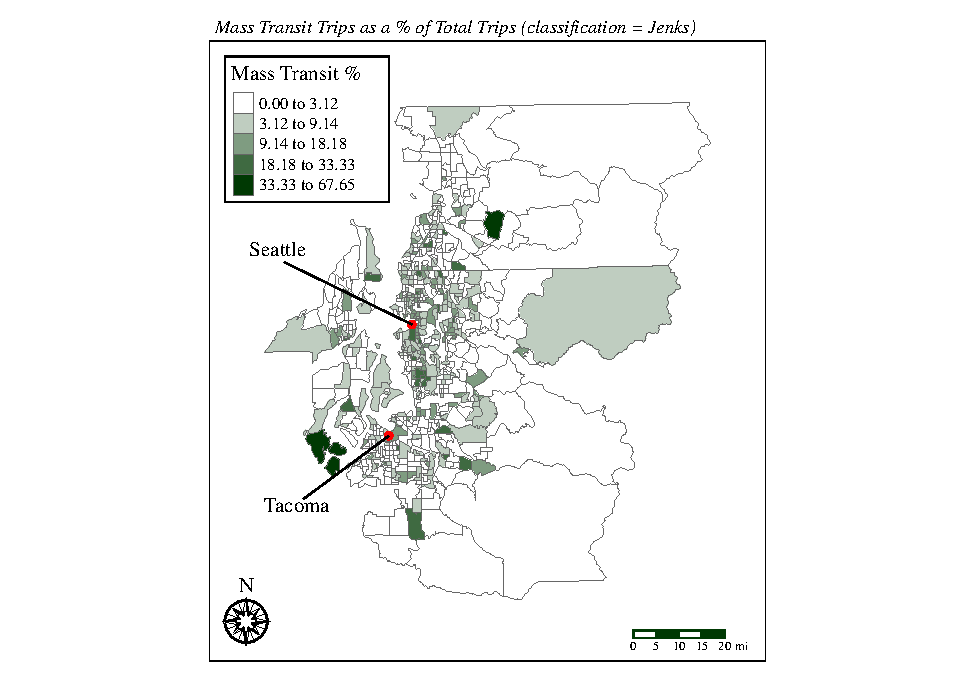
\includegraphics{transit-hotspots-PSRC_files/figure-latex/unnamed-chunk-3-1.pdf}
\caption{Sources: US Census ACS 2022 5-year estimates, Puget Sound
Regional Countil, Cities and Towns of the US 2014, via Stanford
University; Classification = jenks}
\end{figure}

Ignoring for a minute the top-end of the scale, it does seem that there
are some clusters with higher transit usage and that these clusters tend
to exist closer to the cities. Not only can we see that the apparent
clustering occurs nearer to the two cities marked on the map, it also
seems as though smaller census tracts tend to have higher mass transit
percentages. As a general rule of thumb, smaller census tracts tend to
be more urban, so this fits with my hypothesis that transit clustering
will occur in more population dense areas. In the following maps, we can
visually compare the pattern seen in this map to how each of the
predictor variables vary spatially.

\newpage

\begin{figure}
\centering
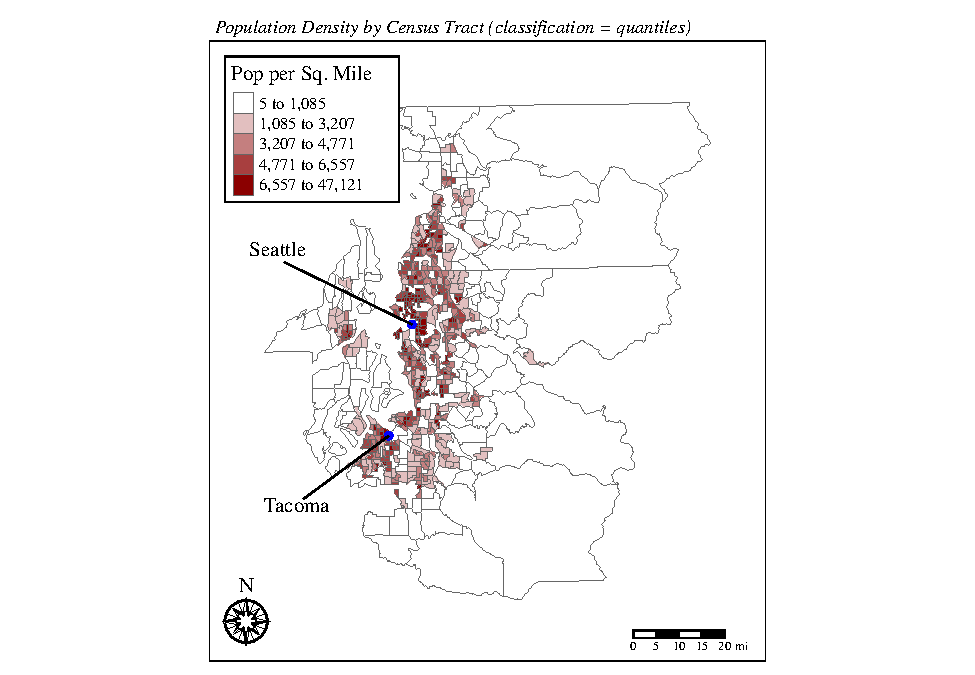
\includegraphics{transit-hotspots-PSRC_files/figure-latex/unnamed-chunk-5-1.pdf}
\caption{Sources: US Census ACS 2022 5-year estimates, Puget Sound
Regional Countil, Cities and Towns of the US 2014, via Stanford
University; Classification = jenks}
\end{figure}

As expected, population density (figure 2) is much higher in tracts
close to the two cities (and throughout the generally-urban corridor
between them). Again, visually comparing this pattern to the one seen
for mass transit percentage, a lot matches up. This is not a perfect
correspondence, of course.

\newpage

\begin{figure}
\centering
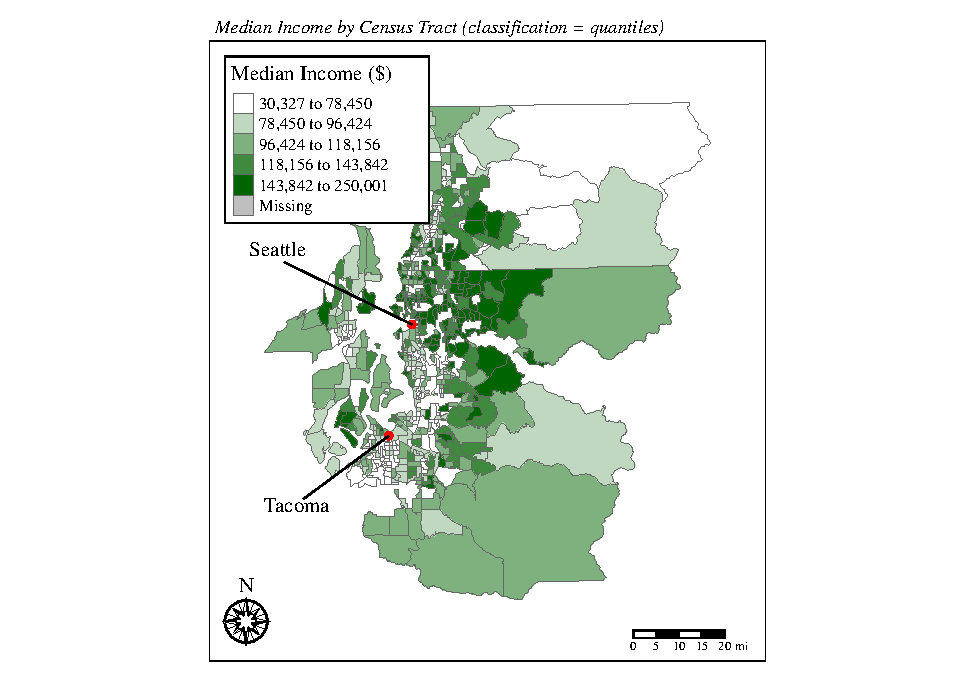
\includegraphics{transit-hotspots-PSRC_files/figure-latex/unnamed-chunk-6-1.pdf}
\caption{Sources: US Census ACS 2022 5-year estimates, Puget Sound
Regional Countil, Cities and Towns of the US 2014, via Stanford
University; Classification = jenks}
\end{figure}

I find the map in figure 3 to be particularly interesting. Although it
is not incredibly easy to compare this spatial pattern to the mass
transit percentage one, I will direct your attention to the high-income
area just East of Seattle. Comparing to the transit map, we can see a
pretty obvious negative association between income and transit
percentage. This provides an initial piece of evidence in favor of the
hypothesis that higher income tracts are likely to have lower transit
usage. In the same vein, a visual inspection of the tracts directly to
the south of the Seattle marker shows an area of comparatively low
median income. Again, cross-referencing this with the transit map, we
can see this is an area of relatively high transit usage.

\newpage

\begin{figure}
\centering
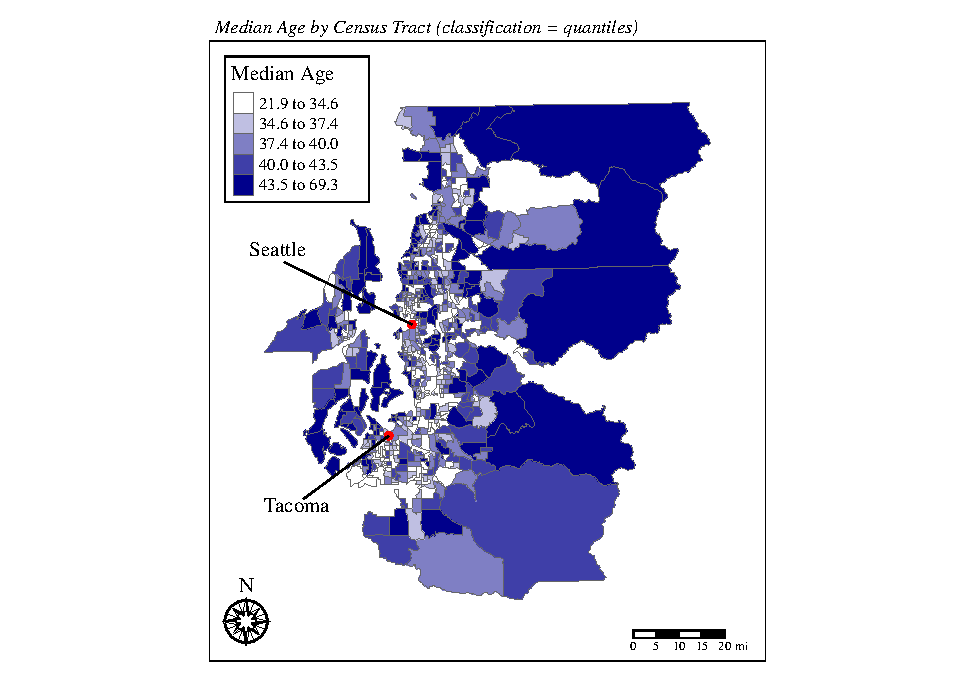
\includegraphics{transit-hotspots-PSRC_files/figure-latex/unnamed-chunk-7-1.pdf}
\caption{Sources: US Census ACS 2022 5-year estimates, Puget Sound
Regional Countil, Cities and Towns of the US 2014, via Stanford
University; Classification = quantiles}
\end{figure}

Finally, another urban/rural pattern can be seen for the median age
variable. Generally speaking, tracts further from the centers of Seattle
and Tacoma tend to be older, while tracts nearer to the cities tend to
be younger. As with the other variables, this provides initial,
non-statistical evidence in support of the idea that tracts with higher
transit ridership should be younger.

For the final piece of exploratory data analysis, below is a table
containing basic descriptive statistics for each of my variables. The
only thing I will call out about this table is that it does show the
high number of tracts with 0\% mass transit trips. This is likely due to
a low number of observations in those census tracts, since I only
filtered out tracts with 0 observations. It is entirely possible there
are tracts with a single observation and that the observation is for
personal vehicles, active transit, or other.

\begin{longtable}[]{@{}lrrrr@{}}
\caption{Descriptive Statistics Summary}\tabularnewline
\toprule\noalign{}
& Mass Transit \% & Population Density & Median Income & Median Age \\
\midrule\noalign{}
\endfirsthead
\toprule\noalign{}
& Mass Transit \% & Population Density & Median Income & Median Age \\
\midrule\noalign{}
\endhead
\bottomrule\noalign{}
\endlastfoot
mean & 5.06 & 4,605.37 & 113,140.27 & 39.19 \\
sd & 6.94 & 4,483.13 & 40,662.76 & 5.69 \\
min & 0.00 & 4.90 & 30,327.00 & 21.90 \\
q25 & 0.00 & 1,779.03 & 84,682.75 & 35.60 \\
median & 2.78 & 3,907.93 & 107,472.00 & 38.70 \\
q75 & 7.69 & 5,963.44 & 135,001.75 & 42.60 \\
max & 67.65 & 47,121.04 & 250,001.00 & 69.30 \\
\end{longtable}

\subsection{Cluster Analysis}\label{cluster-analysis}

In this section, I will apply two different methods to test and
visualize the clustering of transit access in the region. First, I will
run a Global Moran's I to determine if the clustering we can see
visually is statistically significant. Then, I will run a hotspot
analysis using the Getis-Ord Gi* statistic, primarily as a tool for
creating a visualization of the clustering. I will be using the Queen's
case contiguity for my weights, because it intuitively does not make
sense to exclude some neighbors (as would be the case using Rook's case
contiguity) for this research question.

\subsubsection{Moran's I Test of Global
Clustering}\label{morans-i-test-of-global-clustering}

\begin{verbatim}
## 
##  Moran I test under randomisation
## 
## data:  psrc_table_clean$masstransit_perc  
## weights: weights_clean    
## 
## Moran I statistic standard deviate = 7.1199, p-value = 5.4e-13
## alternative hypothesis: greater
## sample estimates:
## Moran I statistic       Expectation          Variance 
##      0.1928134937     -0.0016103060      0.0007456762
\end{verbatim}

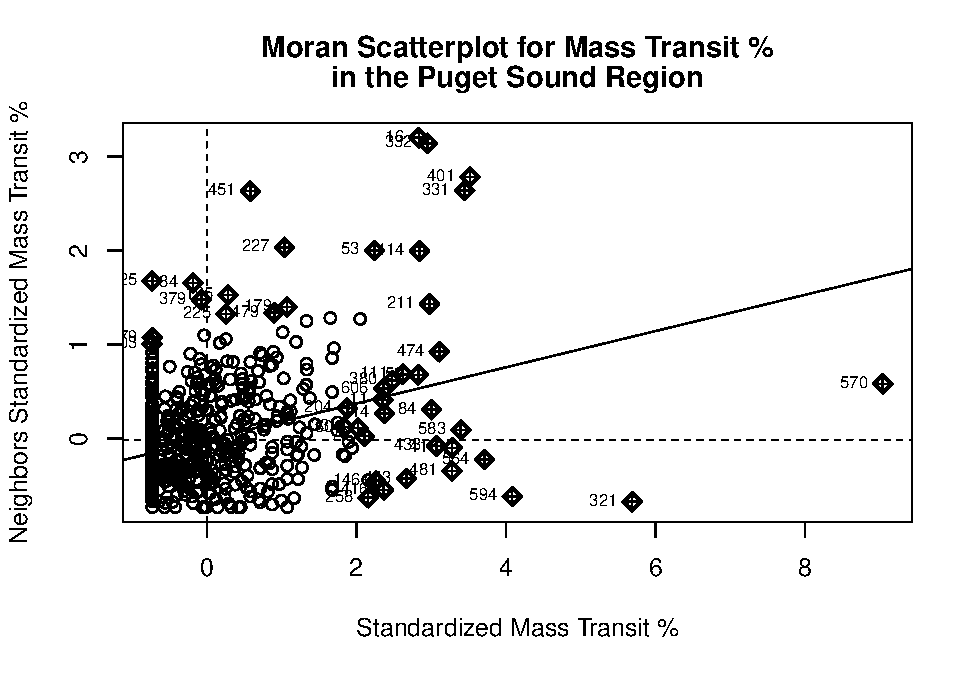
\includegraphics{transit-hotspots-PSRC_files/figure-latex/unnamed-chunk-11-1.pdf}

The Global Moran's I value of 0.193 indicates a moderate, positive
clustering pattern. That is, tracts are somewhat likely to be similar to
their immediate neighbors in terms of their mass transit percentage.
High tracts are likely to be bordered by other high tracts, and low
tracts are likely to be bordered by other low tracts. Given that the
Moran's I statistic ranges from -1 to 1, the 0.193 value only indicates
moderate positive clustering. That said, the p-value associated with
this test is \textless{} 0.001, which makes me confident that this
clustering pattern is not by chance - the likelihood that we would see
this pattern by chance is incredibly low.

While it is useful to know that there is statistically significant
spatial clustering in our variable of interest with the region, these
statistics alone do a poor job of helping us to understand where this
clustering is happening and whether it fits with expectations. To that
end, I will employ the Getis-Ord Gi* statistic and map its values across
the region to visualize mass transit hotspots.

The Moran scatterplot visualizes this moderate positive clustering with
the relatively shallow, positive slope on the plot of standardized mass
transit percentage vs.~neighbors standardized mass transit percentage.

\newpage

\subsubsection{Hotspot Mapping with Getis-Ord
Gi*}\label{hotspot-mapping-with-getis-ord-gi}

The Getis-Ord Gi* statistic evaluates each tract compared to its
neighbors and finds ``hotspots'' (high-value tracts surrounded by other
high-value tracts) and ``coldspots'' (low-value tracts surrounded by
other low-value tracts). The output statistic, is a z-score associated
with each tract. Roughly speaking, Gi* values between -2 and 2 represent
areas with no significant clustering, while values outside that range
(\textless-2 or \textgreater2), represent areas with significant
clustering. A negative Gi* statistic indicates a coldspot, while a
positive Gi* statistic indicates a hotspot. I am using the same spatial
weights matrix as I used for the Global Moran's I.

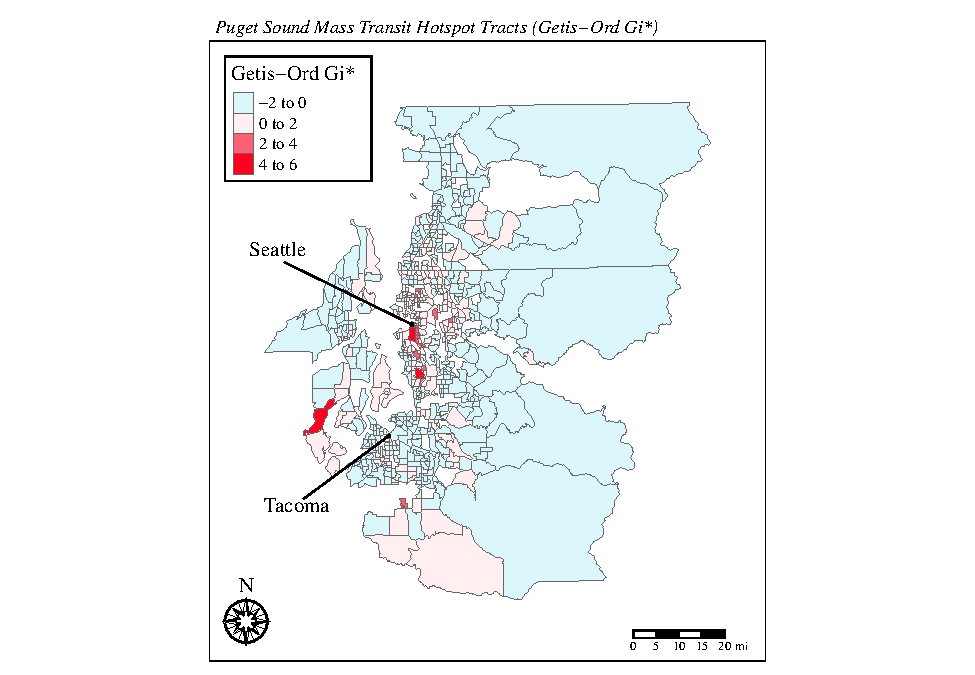
\includegraphics{transit-hotspots-PSRC_files/figure-latex/unnamed-chunk-12-1.pdf}

As can be seen in the map above, I chose to give the tracts with
non-significant Gi* values directional coloration. Tracts with
non-significant negative values are light blue and tracts with
non-significant positive values are light pink. Despite the
non-significance, I do believe this coloration paints a picture
generally consistent with my expectation and thus deserves to be seen,
especially given that sample size is a concern for many of these tracts.

Speaking of significant values, however, it is clear to see that the
predominant occurrences of clustering are nearby Seattle, with most
happening in South Seattle (noted earlier for having high population
density and relatively lower median incomes). There are a couple of
other instances of significant clustering towards the southwest corner
of the map, but I do not have an intuitive explanation for why those are
occurring there. More research on locations of transit lines and tract
characteristics would have to be done in order to get a better
understanding of what is happening.

In the next section, I will take my analysis further with spatial models
that regress mass transit percentage onto the independent variables:
population density, median income, and median age.

\subsection{Regression using Spatial Error Model and Spatial Lag
Model}\label{regression-using-spatial-error-model-and-spatial-lag-model}

\subsubsection{Spatial Lag Model}\label{spatial-lag-model}

First, I will run a spatial lag model, which essentially includes the
value of mass transit percentage in surrounding tracts as defined by the
spatial weights matrix. This allows the model to take into account the
spatial clustering we saw in the Moran's I test and produce coefficients
for the other predictor variables that are more efficient and accurate.
For this testing, I will use the \texttt{lagsarlm()} function from the
\texttt{spatialreg} package. I will log both population density and
median income, which is a common practice for variables that are always
above 0 and can theoretically increase without limit.

\begin{verbatim}
## 
## Call:
## lagsarlm(formula = masstransit_perc ~ log(pop_per_sqmile) + log(medincomeE) + 
##     medageE, data = psrc_table_clean, listw = weights_clean)
## 
## Residuals:
##     Min      1Q  Median      3Q     Max 
## -8.7888 -4.1372 -2.0656  2.3349 61.9643 
## 
## Type: lag 
## Coefficients: (asymptotic standard errors) 
##                      Estimate Std. Error z value Pr(>|z|)
## (Intercept)          0.906643   8.856855  0.1024  0.91847
## log(pop_per_sqmile)  0.491216   0.229086  2.1442  0.03201
## log(medincomeE)     -0.250715   0.777386 -0.3225  0.74707
## medageE              0.038179   0.053273  0.7167  0.47358
## 
## Rho: 0.32971, LR test value: 37.7, p-value: 8.2494e-10
## Asymptotic standard error: 0.049143
##     z-value: 6.7092, p-value: 1.9574e-11
## Wald statistic: 45.013, p-value: 1.9574e-11
## 
## Log likelihood: -2055.995 for lag model
## ML residual variance (sigma squared): 42.829, (sigma: 6.5444)
## Number of observations: 621 
## Number of parameters estimated: 6 
## AIC: 4124, (AIC for lm: 4159.7)
## LM test for residual autocorrelation
## test value: 2.519, p-value: 0.11248
\end{verbatim}

As can be seen in this output, there are two predictors for which the
coefficient is statistically significant. These are the lag term (Rho),
as expected given the clustering already seen above, and the
log(pop\_per\_sqmile) term. The positive coefficient on
log(pop\_per\_sqmile) indicates that greater population density is
associated with greater mass transit percentage. This was hypothesized.
I will not directly try to interpret the values of the coefficients
because the spatial lag term makes direct interpretations inaccurate.
The other predictors are non-significant.

I will also calculate a pseudo \(R^2\) value for this regression model
using the formula \(1 - \frac{SSE}{TSS}\).

\begin{verbatim}
## Pseudo R-squared: 0.1069
\end{verbatim}

This indicates our model explains approximately 10\% of the variation
seen in the dependent variable, mass transit percentage.

\subsubsection{Spatial Error Model}\label{spatial-error-model}

Rather than modeling lag terms, a spatial error model assumes that the
residuals (error) of the model are spatially autocorrelated. It seeks to
address the same issues as the SLM: ensuring the the coefficients and
standard errors for our other predictors are efficient and accurate. I
will use the \texttt{errorsarlm()} function, also via the
\texttt{spatialreg} package.

\begin{verbatim}
## 
## Call:errorsarlm(formula = masstransit_perc ~ log(pop_per_sqmile) + 
##     log(medincomeE) + medageE, data = psrc_table_clean, listw = weights_clean)
## 
## Residuals:
##     Min      1Q  Median      3Q     Max 
## -9.1359 -4.1456 -2.1598  2.4106 61.7270 
## 
## Type: error 
## Coefficients: (asymptotic standard errors) 
##                      Estimate Std. Error z value Pr(>|z|)
## (Intercept)          4.179806  10.937819  0.3821   0.7024
## log(pop_per_sqmile)  0.463804   0.289750  1.6007   0.1094
## log(medincomeE)     -0.352675   0.938844 -0.3756   0.7072
## medageE              0.032458   0.057055  0.5689   0.5694
## 
## Lambda: 0.32786, LR test value: 35.675, p-value: 2.3318e-09
## Asymptotic standard error: 0.049346
##     z-value: 6.6442, p-value: 3.0484e-11
## Wald statistic: 44.146, p-value: 3.0484e-11
## 
## Log likelihood: -2057.008 for error model
## ML residual variance (sigma squared): 42.982, (sigma: 6.5561)
## Number of observations: 621 
## Number of parameters estimated: 6 
## AIC: 4126, (AIC for lm: 4159.7)
\end{verbatim}

Interestingly, none of the predictors in this model are statistically
significant, although the significance in the error term lambda
indicates, once again, that it is important to account for spatial
autocorrelation in our modeling. I will again calculate and print the
pseudo r-squared.

\begin{verbatim}
## Pseudo R-squared: 0.1037
\end{verbatim}

This value is nearly identical to the one for the spatial lag model (as
are the values of log likelihood and AIC), which indicates similar
predictive power between the models.

\section{Discussion and
Interpretation}\label{discussion-and-interpretation}

\subsection{Key Findings}\label{key-findings}

This investigation put into statistical terms a pattern that was (a)
probably easy to intuit and (b) visually apparent from the initial
mapping: high values of transit usage clusters close to city centers
(particularly for Seattle) in the Puget Sound region. A further
corroborating relationship was revealed with the SLM: that population
density is positively associated with mass transit usage.

The other predictor variables (median income and median age) were not
statistically significantly related to my outcome variable. The analysis
did not present me with any surprising or counterintuitive results,
merely a lack of significance for some of my variables.

As an aside, I was interested in how some of the weird variation seen in
areas further outside the city might be affecting my results. I cloned
the R script I used for the analysis and ran all the same analysis, but
filtering to just King country (where Seattle is located), removing
Kitsap, Pierce, and Snohomish counties. Although my regression outputs
remained non-significant (possible reasons why are discussed in the
limitations section below), my clustering statistic became stronger
(still significant) and my regression diagnostics for predictive power
(pseudo \(R^2\), AIC, log likelihood) improved.

\subsection{Implications/Areas for Future
Inquiry}\label{implicationsareas-for-future-inquiry}

With statistical evidence in favor of urban clustering of transit usage,
I can now confidently ask the question: ``what is it about urban areas
that encourages transit ridership?'' I believe this can be decomposed
into two pieces. First, there are likely certain pro-transit
characteristics of urban areas. A high density of stops and transfer
options mean transit is more convenient for riders, as does better
walkability and a lower distance between likely origin and destination.
On the other hand, some characteristics of urban areas have a more
anti-car flavor. Limited and expensive parking options are a good
example. If increasing transit adoption and usage is a priority (and it
should be, for sustainability and equitability reasons), further
research should investigate these characteristics to better understand
how to design desirable transit in areas with low usage rates.

This sort of investigation could remain a spatial one. I imagine a
survey of people in the region, each linked to a census tract, and would
imagine that their public transit usage considerations might vary with
geography. People in urban areas might consider transfer reliability,
walkability, or anti-car factors more than suburban or rural
respondents, who might be more interested in things like overall speed.
Seattle, in particular, has a big suburban population that commutes
either to the city or nearby tech campuses and, as we can see from the
initial choropleth mapping, tends to do so by car. A better
understanding of their reasons for this would allow for better policy
and infrastructure design to increase transit usage and adoption.

\subsection{Limitations}\label{limitations}

There are two major limitations to this analysis. First of all, I have
serious concerns about sample size for this project. As can be seen in
the simple histogram below (binwidth = 30), a large percentage of tracts
have below 30 observations. This gives me concerns about noise. The
structure of my analysis was such that observation count was lost in
translation - my response variable was aggregated and in the form of a
rate. This means that a tract with 5 departures (very likely to be
noisy) was treated the same as one with 1000 departures (unlikely to be
noisy). Missingness is a futher issue with sample size - there are a
number of tracts completely omitted from my analysis because they had no
observations, period. In all honesty, I don't have a great solution for
this off the top of my head, beyond better and more consistent sample
collection.

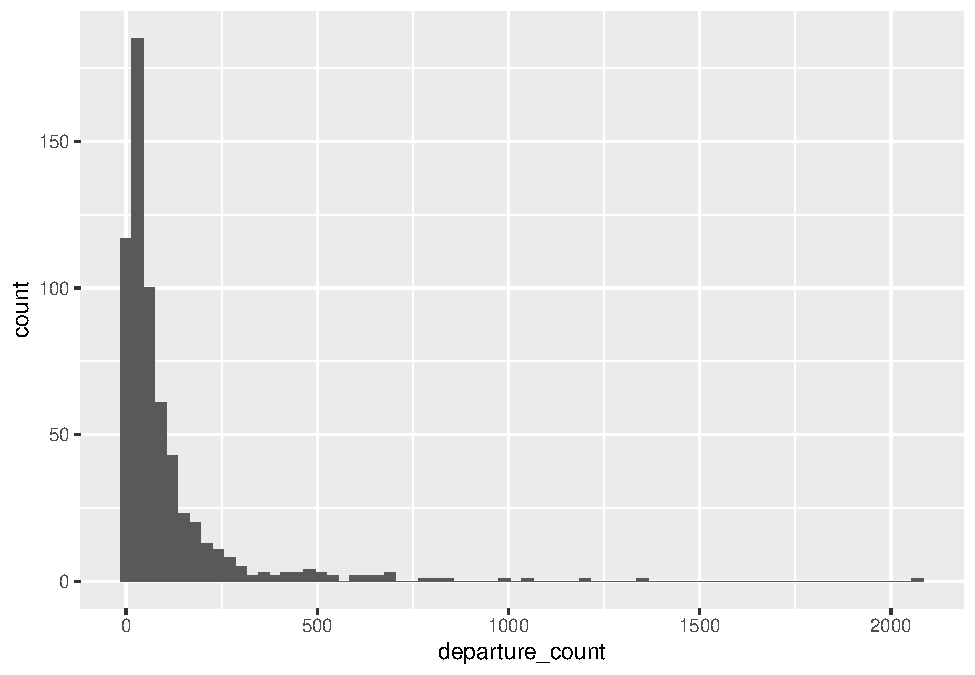
\includegraphics{transit-hotspots-PSRC_files/figure-latex/unnamed-chunk-17-1.pdf}

The second limitation to this analysis (and probably the one more easily
solved) is the lack of predictor variables in my modeling. Given more
time, I would have (a) included more demographic variables and (b)
looked for some built-environment and tract-characteristic variables
(e.g., parking cost, walkability, congestion) to associate with each
tract. Although this would be a time-consuming process, it would add a
lot of color to my model and, at the very least, be likely to improve
the predictive power of my models.

\section{Conclusion}\label{conclusion}

This report can be thought of as a jumping-off point for my personal
research interests. Having this sort of statistical and spatial
understanding of how transit usage is distributed in the region gives me
a concrete foundation off of which to build further analyses. Although I
did not find much in the way of interesting regression results, the
analysis has given me pause to consider what other types of variables
(especially outside of basic ACS demographics) might be useful and/or
interesting to consider adding to future work. Finally, I think the
number of questions that this analysis provokes within me will be
helpful for thinking about future research directions and how the relate
to policy decisions.

\section{References}\label{references}

\subsection{Data Sources}\label{data-sources-1}

\begin{enumerate}
\def\labelenumi{\arabic{enumi}.}
\tightlist
\item
  National Atlas of the United States. (2013). Cities and Towns of the
  United States, 2014. National Atlas of the United States. Available
  at: \url{http://purl.stanford.edu/bx729wr3020}.
\item
  Puget Sound Regional Council. (2023). Household travel survey program.
  Puget Sound Regional Council.
  \url{https://www.psrc.org/our-work/household-travel-survey-program}
\item
  U.S. Census Bureau. (n.d.). \emph{American Community Survey 5-year
  estimates: 2022}. U.S. Department of Commerce. Retrieved December 11,
  2024, from \url{https://data.census.gov/}
\end{enumerate}

\subsection{Programming
Languages/Software}\label{programming-languagessoftware}

\begin{enumerate}
\def\labelenumi{\arabic{enumi}.}
\tightlist
\item
  R Core Team (2024). \emph{R: A Language and Environment for
  Statistical Computing}. R Foundation for Statistical Computing,
  Vienna, Austria. \url{https://www.R-project.org/}.
\item
  RStudio Team. (2020). RStudio: Integrated Development for R. RStudio,
  PBC, Boston, MA. \url{http://www.rstudio.com/}.
\end{enumerate}

\subsection{R Packages}\label{r-packages}

\begin{enumerate}
\def\labelenumi{\arabic{enumi}.}
\tightlist
\item
  Baddeley A, Rubak E, Turner R (2015). \emph{Spatial Point Patterns:
  Methodology and Applications with R}. Chapman and Hall/CRC Press,
  London. ISBN 9781482210200,
  \url{https://www.routledge.com/Spatial-Point-Patterns-Methodology-and-Applications-with-R/Baddeley-Rubak-Turner/p/book/9781482210200/}.
\item
  Bivand R (2022). ``R Packages for Analyzing Spatial Data: A
  Comparative Case Study with Areal Data.'' \emph{Geographical
  Analysis}, \emph{54}(3), 488-518.
  \url{https://doi.org/10.1111/gean.12319}.
\item
  Bivand R, Millo G, Piras G (2021). ``A Review of Software for Spatial
  Econometrics in R.'' \emph{Mathematics}, \emph{9}(11).
  \url{https://doi.org/10.3390/math9111276},
  \url{https://www.mdpi.com/2227-7390/9/11/1276}.
\item
  Bivand R, Pebesma E, Gómez-Rubio V (2013). \emph{Applied spatial data
  analysis with R, Second edition}. Springer, NY.
  \url{https://asdar-book.org/}.
\item
  Bivand R, Wong D (2018). ``Comparing implementations of global and
  local indicators of spatial association.'' \emph{TEST}, \emph{27}(3),
  716-748. \url{https://doi.org/10.1007/s11749-018-0599-x}.
\item
  Müller K (2020). \emph{here: A Simpler Way to Find Your Files}. R
  package version 1.0.1, \url{https://CRAN.R-project.org/package=here}.
\item
  Pebesma, E., \& Bivand, R. (2023). Spatial Data Science: With
  Applications in R. Chapman and Hall/CRC.
  \url{https://doi.org/10.1201/9780429459016}
\item
  Pebesma E, Bivand R (2023). \emph{Spatial Data Science With
  Applications in R}. Chapman \& Hall.
  \url{https://r-spatial.org/book/}.
\item
  Pebesma, E., 2018. Simple Features for R: Standardized Support for
  Spatial Vector Data. The R Journal 10 (1), 439-446,
  \url{https://doi.org/10.32614/RJ-2018-009}
\item
  Tennekes M (2018). ``tmap: Thematic Maps in R.'' \emph{Journal of
  Statistical Software}, \emph{84}(6), 1-39.
  \url{https://doi.org/10.18637/jss.v084.i06}.
\item
  Walker K, Herman M (2024). \emph{tidycensus: Load US Census Boundary
  and Attribute Data as `tidyverse' and `sf'-Ready Data Frames}. R
  package version 1.6.7,
  \url{https://CRAN.R-project.org/package=tidycensus}.
\item
  Wickham H (2023). \emph{forcats: Tools for Working with Categorical
  Variables (Factors)}. R package version 1.0.0,
  \url{https://CRAN.R-project.org/package=forcats}.
\item
  Wickham H, Averick M, Bryan J, Chang W, McGowan LD, François R,
  Grolemund G, Hayes A, Henry L, Hester J, Kuhn M, Pedersen TL, Miller
  E, Bache SM, Müller K, Ooms J, Robinson D, Seidel DP, Spinu V,
  Takahashi K, Vaughan D, Wilke C, Woo K, Yutani H (2019). ``Welcome to
  the tidyverse.'' \emph{Journal of Open Source Software}, \emph{4}(43),
  1686. \url{https://doi.org/10.21105/joss.01686}.
\item
  Xie Y (2024). \emph{knitr: A General-Purpose Package for Dynamic
  Report Generation in R}. R package version 1.48,
  \url{https://yihui.org/knitr/}.
\item
  Yihui Xie (2015) Dynamic Documents with R and knitr. 2nd edition.
  Chapman and Hall/CRC. ISBN 978-1498716963
\item
  Yihui Xie (2014) knitr: A Comprehensive Tool for Reproducible Research
  in R. In Victoria Stodden, Friedrich Leisch and Roger D. Peng,
  editors, Implementing Reproducible Computational Research. Chapman and
  Hall/CRC. ISBN 978-1466561595
\end{enumerate}

\end{document}
